\appendix

\section{Identification of the lines and measurement of the absorption}

\begin{table}[H]
\centering
\caption{Data from the measurement of the 39 peaks in the NH$_3$ spectrum. The error of the absorption coefficients have been determent with error propagation. The experted values are taken from \cite{examenarbeit}}
\label{tab:data_39_1}
\begin{tabular}{c|c|c|c|c|c|c|c|c}
 Nummer &   J &   K &  $\nu_{theo}$ &  $\nu_{gemessen}$ &  Amplitude &   err &  absorptionskoeffizient &  absorp\_err \\ \hline
      1 &   7 &   3 &   18.058 &       18.028 &      0.22 &  0.01 &                0.01 &    0.01 \\
      2 &  10 &   7 &   18.282 &       18.294 &      0.10 &  0.01 &                0.006 &    0.001 \\
      3 &   6 &   1 &   18.382 &       18.395 &      0.09 &  0.01 &                0.006 &    0.001 \\
      4 &   9 &   6 &   18.495 &       18.509 &      0.4 &  0.01 &                0.026 &    0.001 \\
      5 &   8 &   5 &   18.819 &       18.819 &      0.5 &  0.01 &                0.029 &    0.001 \\
      6 &   6 &   2 &   18.879 &       18.891 &      0.3 &  0.01 &                0.020 &    0.001 \\
      7 &   7 &   4 &   19.216 &       19.225 &      0.2 &  0.01 &                0.01 &    0.01 \\
      8 &   6 &   3 &   19.735 &       19.764 &      1.4 &  0.1 &                0.09 &    0.01 \\
      9 &   5 &   1 &   19.836 &       19.842 &      0.10 &  0.01 &                0.01 &    0.01 \\
     10 &   5 &   2 &   20.371 &       20.378 &      1.3 &  0.1 &                0.08 &    0.01 \\
     11 &   8 &   6 &   20.722 &       20.721 &      2.4 &  0.1 &                0.15 &    0.01 \\
     12 &   9 &   7 &   20.739 &       20.739 &      0.83 &  0.01 &                0.05 &    0.01 \\
     13 &   7 &   5 &   20.806 &       20.809 &      1.4 &  0.1 &                0.09 &    0.01 \\
     14 &  10 &   8 &   20.857 &       20.855 &      0.26 &  0.01 &                0.016 &    0.01 \\
     15 &   6 &   4 &   20.996 &       20.999 &      1.6 &  0.1 &                0.10 &    0.01 \\
     16 &  11 &   9 &   21.076 &       21.076 &      0.30 &  0.01 &                0.02 &    0.01 \\
     17 &   4 &   1 &   21.134 &       21.140 &      2.7 &  0.1 &                0.17 &    0.01 \\
     18 &   5 &   3 &   21.293 &       21.290 &      4.7 &  0.1 &                0.28 &    0.01 \\
     19 &   4 &   2 &   21.704 &       22.703 &      3.4 &  0.1 &                0.21 &    0.01 \\
     20 &   3 &   1 &   22.235 &       22.240 &      2.7 &  0.1 &                0.17 &    0.01 \\
\end{tabular}
\end{table}

\begin{table}[H]
\centering
\caption{Data from the measurement of the 39 peaks in the NH$_3$ spectrum. The error of the absorption coefficients have been determent with error propagation. The experted values are taken from \cite{examenarbeit}}
\label{tab:data_39_2}
\begin{tabular}{c|c|c|c|c|c|c|c|c}
 Nummer &   J &   K &  $\nu_{theo}$ &  $\nu_{gemessen}$ &  Amplitude &   err &  absorptionskoeffizient &  absorp\_err \\ \hline
     21 &   5 &   4 &   22.654 &       22.660 &     10.2 &  0.1 &                0.572 &    0.009 \\
     22 &   4 &   3 &   22.687 &       22.695 &     14.7 &  0.1 &                0.780 &    0.008 \\
     23 &   6 &   5 &   22.734 &       22.735 &      6.0 &  0.1 &                0.36 &    0.01 \\
     24 &   3 &   2 &   22.835 &       22.835 &      5.7 &  0.1 &                0.34 &    0.01 \\
     25 &   7 &   6 &   22.927 &       22.929 &      8.6 &  0.1 &                0.492 &    0.009 \\
     26 &   2 &   1 &   23.099 &       23.110 &      3.6 &  0.1 &                0.22 &    0.01 \\
     27 &   8 &   7 &   23.235 &       23.239 &      5.0 &  0.1 &                0.30 &    0.01 \\
     28 &   9 &   8 &   23.660 &       23.662 &      4.6 &  0.1 &                0.28 &    0.01 \\
     29 &   1 &   1 &   23.694 &       23.700 &      9.2 &  0.1 &                0.520 &    0.009 \\
     30 &   2 &   2 &   23.723 &       23.730 &      9.7 &  0.1 &                0.547 &    0.009 \\
     31 &   3 &   3 &   23.870 &       23.877 &     20.0 &  0.1 &                1.000 &    0.007 \\
     32 &   4 &   4 &   24.139 &       24.140 &     15.1 &  0.1 &                0.797 &    0.008 \\
     33 &  10 &   9 &   24.208 &       24.206 &      6.1 &  0.1 &                0.36 &    0.01 \\
     34 &   5 &   5 &   24.533 &       24.538 &     14.5 &  0.1 &                0.771 &    0.008 \\
     35 &  11 &  10 &   24.883 &       24.859 &      2.0 &  0.1 &                0.12 &    0.01 \\
     36 &   6 &   6 &   25.056 &       25.061 &     19.7 &  0.1 &                0.988 &    0.007 \\
     37 &  12 &  11 &   25.694 &       25.699 &      2.0 &  0.1 &                0.13 &    0.01 \\
     38 &   7 &   7 &   25.715 &       25.714 &     11.1 &  0.1 &                0.615 &    0.009 \\
     39 &   8 &   8 &   26.519 &       26.523 &      7.8 &  0.1 &                0.45 &    0.01 \\
\end{tabular}
\end{table}


\section{Hyperfine structure}
\label{sec:hf_anhang}


\begin{table}[H]
\centering
\caption{Parameter form the fit, for the hyperfine structure. $\mu$ is given in ms}
\label{tab:hf_6_6_data}
\begin{tabular}{c|c|c}
 Peak & 3 3 & 4 4 \\ \hline
$\mu_1$ &		1.608(2)  	&  	2.12(4)	\\ 
$\mu_2$ &  		1.721(2)	&  	2.21(5)	\\ 
$\mu_3$ &  		2.0011(1)	&  	2.59(3)	\\ 
$\mu_4$ &  		2.289(2)	&  	2.98(5)	\\ 
$\mu_5$ &  		2.401(2)	& 	3.11(5)	\\ 
$\chi^2_{red}$ & 0.94		& 	22.01	\\
\end{tabular} 
\end{table}



\begin{figure}[H]
\centering
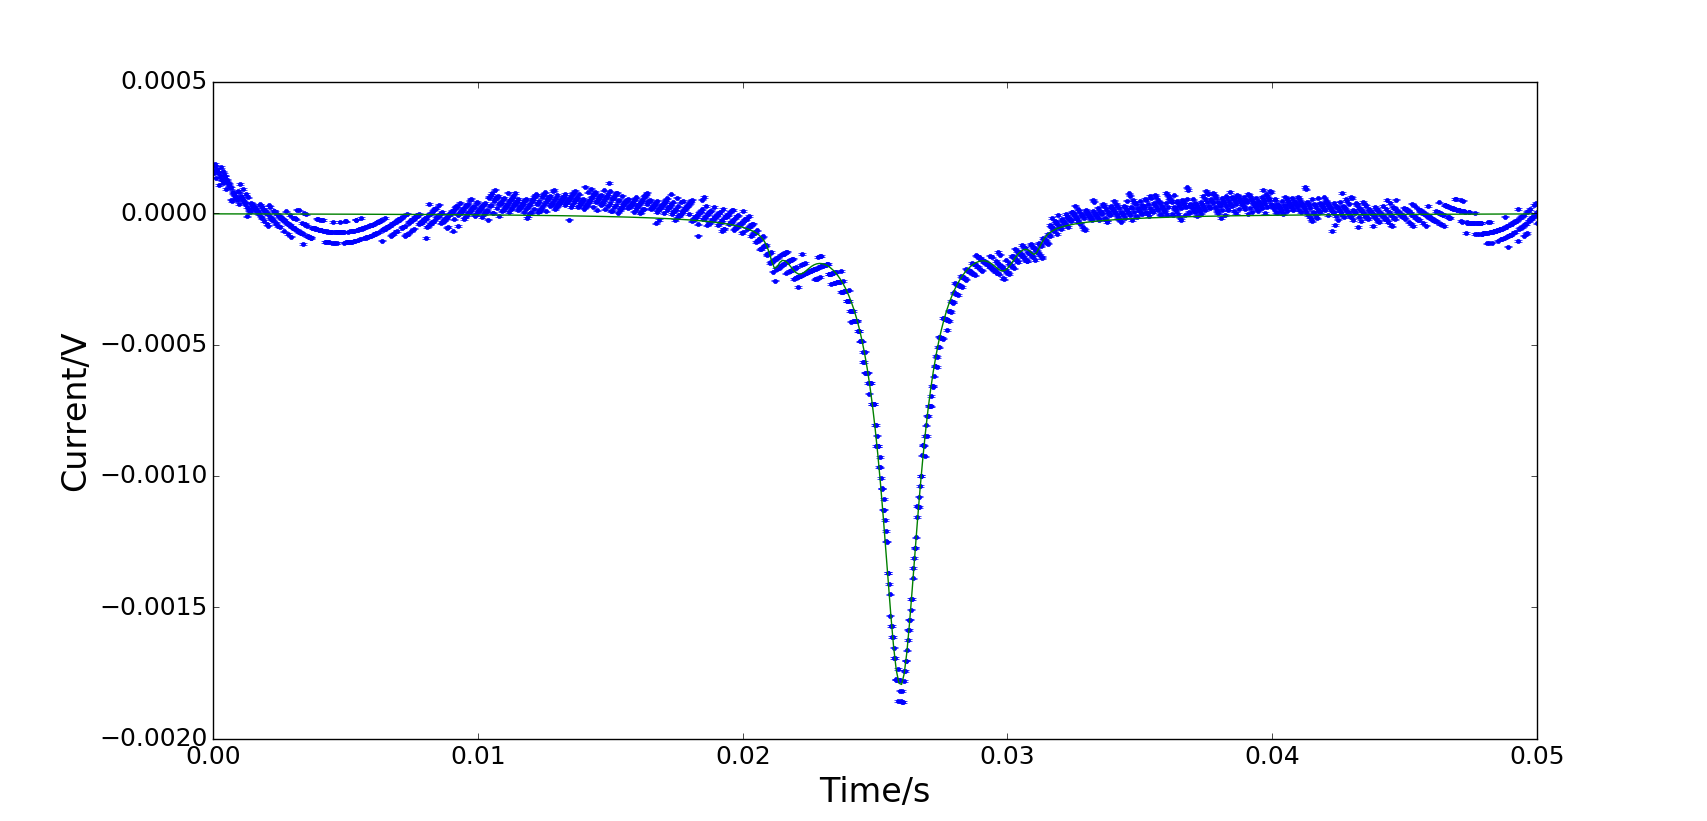
\includegraphics[scale = 0.39]{hf_4_4.png}
\caption{Plot of the 4 4 Peak with the fit for the hyperfine structure. The hyperfine structure is barley visible}
\label{fig:hf_4_4} 
\end{figure}
